{\usebackgroundtemplate{
    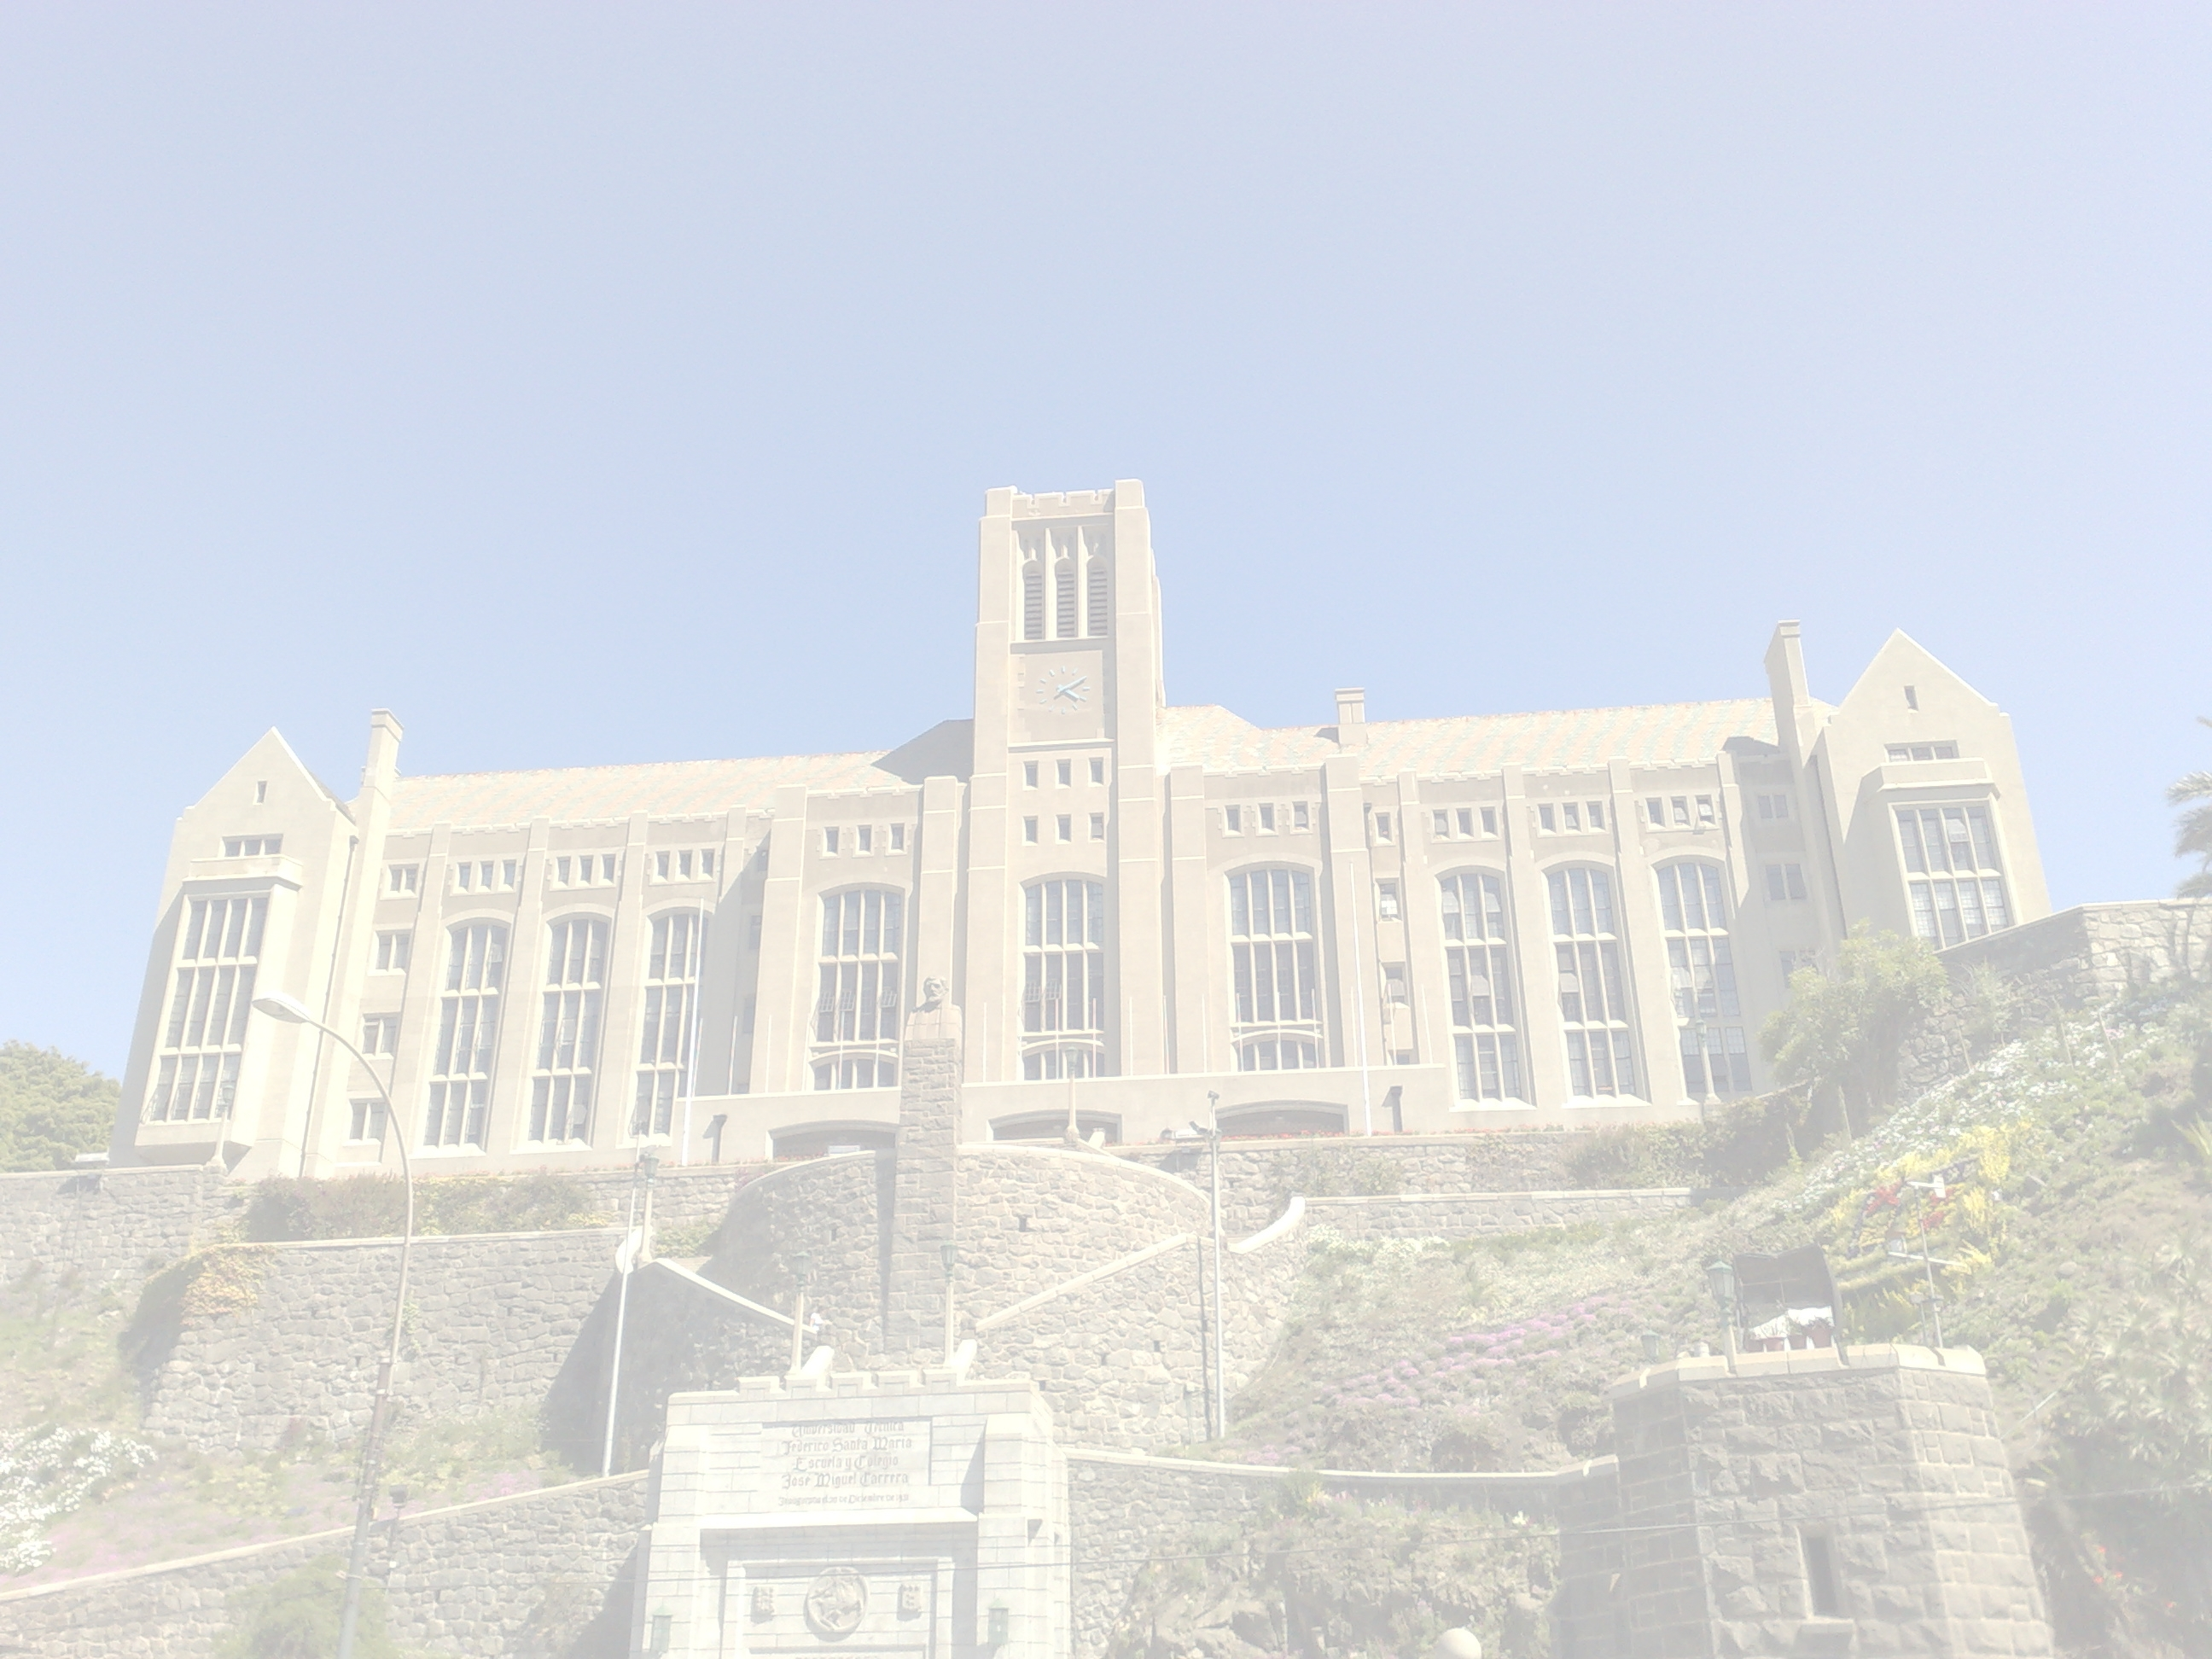
\includegraphics[width=\paperwidth,
      height=\paperheight]{Pict/UTFSM-30.jpg}
  }
  \begin{frame}
    \titlepage
  \end{frame}
}


\begin{frame}
  \frametitle{Outline of the Course}
  \begin{itemize}
  \item Review of geometry on $\R^n$.
  \item Manifolds and Bundles.
  \item Differential Forms.
  \end{itemize}
\end{frame}


\begin{frame}[t]
  \frametitle{Geometric Objects}
  Let $F$ be a function,      $F:\R^n\to\R^m$.
  \begin{columns}[t]
    \column{.5\textwidth}
    \begin{itemize}
    \item \alert{ Scalar}:
      \begin{align*}
        F:\R^n \to \R
      \end{align*}
      \begin{example}
        Temperature in space
      \end{example}
      \item \alert{Vector}:
      \begin{align*}
        F:\R^n \to \R^n
      \end{align*}
      \begin{example}
        Electric field in space
      \end{example}
    \end{itemize}
    \column{.5\textwidth}
    \begin{center}
      \tdplotsetmaincoords{70}{110}
      \begin{tikzpicture}[tdplot_main_coords]
        \draw[thick,->] (0,0,0) -- (2,0,0) node[anchor=north east]{$x$};
        \draw[thick,->] (0,0,0) -- (0,2,0) node[anchor=north west]{$y$};
        \draw[thick,->] (0,0,0) -- (0,0,2) node[anchor=south]{$z$};
        \coordinate (O) at (0,0,0);
        \coordinate (p) at (1,1.5,1.5);
        \draw[->,color=blue,dashed] (O) -- (p);
        \draw[fill=red!80!black,thick]  (p) circle (.4mm) node[anchor=south west] {$T$} node[anchor=north] {$p$};
        %\draw[->]
      \end{tikzpicture}
      \begin{tikzpicture}[tdplot_main_coords]
        \draw[thick,->] (0,0,0) -- (2,0,0) node[anchor=north east]{$x$};
        \draw[thick,->] (0,0,0) -- (0,2,0) node[anchor=north west]{$y$};
        \draw[thick,->] (0,0,0) -- (0,0,2) node[anchor=south]{$z$};
        \coordinate (O) at (0,0,0);
        \coordinate (p) at (1,1.5,1.5);
        \draw[->,color=blue,dashed] (O) -- (p);
        \draw[fill=red!80!black,thick]  (p) circle (.4mm)  node[anchor=north] {$p$};
        \draw[very thick,->,color=yellow!80!black] (p) -- (1.5,1,2.5) node[midway,above,sloped] {$\vec{E}$};
      \end{tikzpicture}
    \end{center}
  \end{columns}
\end{frame}

\begin{frame}
  \frametitle{More Geometric Objects}
  \begin{alertblock}{Plenty of them!}
    There exist examples with $m\neq1$ or $m\neq n$.
  \end{alertblock}
  \begin{columns}
    \column{.5\textwidth}
    Consider a linear array of spins.
    \begin{center}
      \tdplotsetmaincoords{60}{140}
      \begin{tikzpicture}[tdplot_main_coords]
        \draw[very thin,dash pattern=on5pt off3pt] (0,-3,0) -- (0,3,0);
        \foreach \y in {-2,...,2}
        \draw[fill=red!80!black,thick]  (0,\y,0) circle (.4mm)  node[anchor=north] {$p_{\y}$};
        %% \foreach \x in {-2,...,2}
        \draw[very thick,color=green!70!black,->] (0,-2,0) -- (.2,-2.3,.1);
        \draw[very thick,color=green!70!black,->] (0,-1,0) -- (-.2,-0.8,.2);
        \draw[very thick,color=green!70!black,->] (0,0,0) -- (.1,.1,-.1);
        \draw[very thick,color=green!70!black,->] (0,1,0) -- (-.1,.9,-.2);
        \draw[very thick,color=green!70!black,->] (0,2,0) -- (.2,2.3,-.1);
      \end{tikzpicture}
    \end{center}
    \column{.5\textwidth}
    \begin{block}{What object would describe it?}
      Given a point in a line one obtain an arrow. It is described by a function $F:\R\to\R^3$.
    \end{block}
    \begin{itemize}
    \item It's not a scalar in $\R$.
    \item It's not a vector in $\R^3$.
    \alert{
    \item What }is it?
    \alert{
    \item How} does one properly define them?
    \end{itemize}
  \end{columns}
\end{frame}

\begin{frame}[t]
  \frametitle{Transformations}
    \begin{center}
      \begin{tikzpicture}
        % Definitions
        \pgfmathsetmacro{\rp}{2}
        \pgfmathsetmacro{\be}{50}
        \pgfmathsetmacro{\th}{20}
        \pgfmathsetmacro{\px}{\rp*cos(\be)}
        \pgfmathsetmacro{\py}{\rp*sin(\be)}
        \pgfmathsetmacro{\al}{\be-\th}
        \pgfmathsetmacro{\xa}{\rp*cos(\be)}
        \pgfmathsetmacro{\ya}{\rp*sin(\be)}
        \pgfmathsetmacro{\xb}{\rp*cos(\al)}
        \pgfmathsetmacro{\yb}{\rp*sin(\al)}

        % Coordinates
        \coordinate (O) at (0,0);
        \coordinate (P) at (\px,\py);

        % Draw O coordinate system
        \draw[thick,->] (O) -- (0:3cm) node[anchor=north west] {$x$};
        \draw[thick,->] (O) -- (90:3cm) node[anchor=south] {$y$};

        % Draw O' coordinate system
        \draw[thick,->,color=blue] (O) -- (\th:3cm) node[anchor=north west] {$x$};
        \draw[thick,->,color=blue] (O) -- (\th+90:3cm) node[anchor=south] {$y$};

        % Draw the point with line
        \draw[fill=red!80!black,thick]  (P) circle (.4mm) node[anchor=south west] {$p$};
        \draw[color=red!80!black,thick,->] (O) -- (P);

        % Projection to O system
        \draw[thin,dashed] (P) -- (\xa,0) node[anchor=north] {$x_p$};
        \draw[thin,dashed] (P) -- (0,\ya) node[anchor=east] {$y_p$};

        % Projection to O' system
        \draw[thin,dashed,color=blue] (P) -- (\th:\xb) node[anchor=north west] {${x'}_p$};
        \draw[thin,dashed,color=blue] (P) -- (\th+90:\yb) node[anchor=north east] {${y'}_p$};

        % Arcs
        \draw[left color=red!30, right color=red!15,draw=red!60!black] (O) -- (\th:8mm) arc (\th:\be:8mm)  -- cycle;
        \draw (O) +(35:8mm) node[color=red,anchor=south west]  {$\alpha$};
        \draw[left color=blue!30, right color=blue!15,draw=blue!60!black] (O) -- (0:8mm) arc (0:\th:8mm)  -- cycle;
        \node[anchor=west,color=blue] at (\th*2/3:8mm) {$\theta$};

        % Information box
        \draw[xshift=35mm,yshift=15mm] node[right,text width=6cm,rounded corners,fill=red!10,draw=red!40!yellow,inner sep=1ex] {
          \begin{align*}
            x_p = & r_p \cos(\theta+\alpha) \\
            = &x'_p \cos(\theta) - y'_p\sin(\theta)\\
            y_p = & r_p \sin(\theta+\alpha) \\
            = & x'_p \sin(\theta) - y'_p\cos(\theta)
          \end{align*}
        };
      \end{tikzpicture}
    \end{center}
  \begin{columns}
    \column{.5\textwidth}
    {\small
      \begin{align*}
        \begin{pmatrix}
          x'_p\\ y'_p
        \end{pmatrix} = 
        \begin{pmatrix}
          \cos(\theta) & \sin(\theta)\\
          -\sin(\theta) & \cos(\theta)
        \end{pmatrix}
        \begin{pmatrix}
          x_p\\ y_p
        \end{pmatrix}
      \end{align*}
    }
    \column{.5\textwidth}
    In general,
    \begin{align*}
      X' = R(\theta) X,
    \end{align*}
    where $\{R(\theta)\}$ form a \alert{group} of transformations
  \end{columns}
\end{frame}

\begin{frame}[t]
  \frametitle{Definitions from transformations}
  It make sense to define \alert{geometrical objects} depending of their transformation rules of a given group.
  \begin{definition}%{Scalar}
    A {\bf \alert{scalar}} (of a group) is the quantity that remain invariable under the transformation group.
    \begin{align*}
      \Phi' = \Phi
    \end{align*}
  \end{definition}
  \pause
  \begin{alertblock}{R\^ole of group theory}
    \begin{itemize}%[<+->]
    \item One might assign a geometrical object to any irrep of a group.
    \item A scalar is the corresponding to the trivial representation.
    \item A vector is the corresponding to the \alert{fundamental} representation.
    \end{itemize}
  \end{alertblock}
\end{frame}


\begin{frame}
  \frametitle{Definition of Vector}
  \begin{definition}
    A \alert{vector} (of a group) is the quantity that transform under the fundamental representation of the group, i.e.,
    \begin{align*}
      V' = \Lambda V.
    \end{align*}
  \end{definition}
  \begin{alertblock}{Warning}
    \begin{itemize}
    \item $\R^n$ is so simple that is not a good example.
    \item $\R^n$ is the basis for more complex examples.
    \item There are more than `a' vector space.
    \end{itemize}
  \end{alertblock}
\end{frame}


\begin{frame}
  \frametitle{Graphical Representation of Scalar Transf.}
  \begin{center}
    \begin{tikzpicture}
      % Definitions
        \pgfmathsetmacro{\rp}{2}
        \pgfmathsetmacro{\be}{50}
        \pgfmathsetmacro{\th}{20}
        \pgfmathsetmacro{\px}{\rp*cos(\be)}
        \pgfmathsetmacro{\py}{\rp*sin(\be)}
        \pgfmathsetmacro{\al}{\be-\th}
        \pgfmathsetmacro{\xa}{\rp*cos(\be)}
        \pgfmathsetmacro{\ya}{\rp*sin(\be)}
        \pgfmathsetmacro{\xb}{\rp*cos(\al)}
        \pgfmathsetmacro{\yb}{\rp*sin(\al)}

        % Coordinates
        \coordinate (O) at (0,0);
        \coordinate (P) at (\px,\py);

        % Draw O coordinate system
        \draw[thick,->] (O) -- (0:3cm) node[anchor=north west] {$x$};
        \draw[thick,->] (O) -- (90:3cm) node[anchor=south] {$y$};

        % Draw O' coordinate system
        \draw[thick,->,color=blue] (O) -- (\th:3cm) node[anchor=north west] {$x$};
        \draw[thick,->,color=blue] (O) -- (\th+90:3cm) node[anchor=south] {$y$};

        % Draw the point with line
        \draw[fill=red!80!black,thick]  (P) circle (.4mm) node[anchor=south west] {$p$};
        \draw[color=red!80!black,thick,->] (O) -- (P);

        % Projection to O system
        \draw[thin,dashed] (P) -- (\xa,0) node[anchor=north] {$x_p$};
        \draw[thin,dashed] (P) -- (0,\ya) node[anchor=east] {$y_p$};

        % Projection to O' system
        \draw[thin,dashed,color=blue] (P) -- (\th:\xb) node[anchor=north west] {${x'}_p$};
        \draw[thin,dashed,color=blue] (P) -- (\th+90:\yb) node[anchor=north east] {${y'}_p$};

        % Information box
        \draw[xshift=35mm,yshift=15mm] node[right,text width=6cm,rounded corners,fill=red!10,draw=red!40!yellow,inner sep=1ex] {
          In $S$ there is a function $f(x)$, while in $S'$ there is a $f'(x')$.
          \begin{align*}
            f'(x') = f'\(\Lambda x\) = & f(x)\\
            \text{or}\quad f'\(x\) = & f\(\Lambda^{-1} x\).
          \end{align*}
        };
    \end{tikzpicture}
  \end{center}
\end{frame}

\begin{frame}
  \frametitle{Graphical Representation of Vector Transf.}
  \begin{center}
    \begin{tikzpicture}
      % Definitions
        \pgfmathsetmacro{\rp}{2}
        \pgfmathsetmacro{\be}{50}
        \pgfmathsetmacro{\th}{20}
        \pgfmathsetmacro{\px}{\rp*cos(\be)}
        \pgfmathsetmacro{\py}{\rp*sin(\be)}
        \pgfmathsetmacro{\al}{\be-\th}
        \pgfmathsetmacro{\xa}{\rp*cos(\be)}
        \pgfmathsetmacro{\ya}{\rp*sin(\be)}
        \pgfmathsetmacro{\xb}{\rp*cos(\al)}
        \pgfmathsetmacro{\yb}{\rp*sin(\al)}

        % Coordinates
        \coordinate (O) at (0,0);
        \coordinate (P) at (\px,\py);

        % Draw O coordinate system
        \draw[thick,->] (O) -- (0:3cm) node[anchor=north west] {$x$};
        \draw[thick,->] (O) -- (90:3cm) node[anchor=south] {$y$};

        % Draw O' coordinate system
        \draw[thick,->,color=blue] (O) -- (\th:3cm) node[anchor=north west] {$x$};
        \draw[thick,->,color=blue] (O) -- (\th+90:3cm) node[anchor=south] {$y$};

        % Draw the point with line
        \draw[fill=red!80!black,thick]  (P) circle (.4mm) node[anchor=south west] {$p$};
        \draw[color=red!80!black,thick,->] (O) -- (P);

        % Projection to O system
        \draw[thin,dashed] (P) -- (\xa,0) node[anchor=north] {$x_p$};
        \draw[thin,dashed] (P) -- (0,\ya) node[anchor=east] {$y_p$};

        % Projection to O' system
        \draw[thin,dashed,color=blue] (P) -- (\th:\xb) node[anchor=north west] {${x'}_p$};
        \draw[thin,dashed,color=blue] (P) -- (\th+90:\yb) node[anchor=north east] {${y'}_p$};

        % Draw the vector
        \draw[very thick,color=yellow!75!black,->] (P) -- +(110:1cm) node[anchor=south west,color=black] {$\vec{V}$};

        % Information box
        \draw[xshift=35mm,yshift=15mm] node[right,text width=6cm,rounded corners,fill=red!10,draw=red!40!yellow,inner sep=1ex] {
          In $S$ there is a vector $\vec{V}(x)$, while in $S'$ there is a $\vec{V}'(x')$.
          \begin{align*}
            \vec{V}'(x') = \vec{V}'\(\Lambda x\) = & \Lambda\vec{V}(x)\\
            \text{or}\quad \vec{V}'\(x\) = & \Lambda\vec{V}\(\Lambda^{-1} x\).
          \end{align*}
        };
    \end{tikzpicture}
  \end{center}
\end{frame}


\begin{frame}
  \frametitle{Vectors in $\R^n$}
  \begin{columns}
    \column{.5\textwidth}
    \begin{itemize}
    \item {\bf Basis:} $\vec{e}_i$ with $i\in\{1,...,n\}$.
    \item {\bf Vector:} $\vec{V} = \sum_i V^i \vec{e}_i$.
    \item Vectors might be seen as arrows in $\R^n$.
    \end{itemize}
    \column{.5\textwidth}
    \begin{center}
      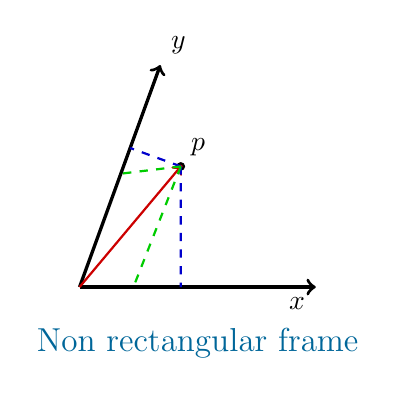
\begin{tikzpicture}
        % Definition
        \pgfmathsetmacro{\rp}{2}
        \pgfmathsetmacro{\th}{50}
        \pgfmathsetmacro{\ph}{20}
        \pgfmathsetmacro{\xa}{\rp*cos(\th)}
        \pgfmathsetmacro{\xb}{\rp*sin(90-\th-\ph)}
        \pgfmathsetmacro{\yb}{\rp*sin(\th)}
        \pgfmathsetmacro{\ya}{\rp*cos(90-\th-\ph)}

        % Coordinates
        \coordinate (O) at (0,0);
        \coordinate (P) at (\th:\rp cm);

        % Draw the frame
        \draw[very thick,->] (O) -- (0:3cm) node[anchor=north east] {$x$};
        \draw[very thick,->] (O) -- (90-\ph:3cm) node[anchor= south west] {$y$};

        % Draw point  with line
        \draw[fill=red!80!black,thick]  (P) circle (.4mm) node[anchor=south west] {$p$};
        \draw[color=red!80!black,thick,->] (O) -- (P);

        % Draw projections
        \draw[thick,dashed,color=blue!80!black] (P) -- (\xa,0);
        \draw[dashed,thick,color=blue!80!black] (P) -- (90-\ph:\ya);
         \draw[dashed,thick,color=green!80!black] (P) -- (\xb,0);
        \draw[dashed,thick,color=green!80!black] (P) -- (90-\ph:\yb);

        % Title
        \node[anchor=north,color=green!40!blue] at (current bounding box.south) {{\large Non rectangular frame}};       
      \end{tikzpicture}
    \end{center}
  \end{columns}
  \begin{alertblock}{Different vectors}
    \begin{itemize}
    \item Covariant and
    \item Contravariant.
    \end{itemize}
  \end{alertblock}
\end{frame}


\begin{frame}
  \frametitle{Notation(s)}
  \begin{center}
    \begin{tabular}{|>{\columncolor{red!10}\color{blue}}c|>{\columncolor{yellow!15}}c|>{\columncolor{yellow!15}}c|}
      \hline
      \rowcolor[gray]{0.9}& Vectors & Covectors\\
      \hline\hline
      Basis & A set $\{\vb{i}\}$ & A set $\{\fb{i}\}$\\
      Vector &  $\vec{V}= \sum_i \; V^i\vb{i}$ &  $\widetilde{V}= \sum_i \; V_i\fb{i}$ \\
      & $V^i$  & $V_i$ \\
      QM Basis & A set $\{\ket{i}\}$ &A set $\{\bra{i}\}$  \\
      QM Vector & $\ket{V} = \sum_i V^i\ket{i}$ &  $\bra{V} = \sum_i V_i\bra{i}$\\
      \hline
    \end{tabular}
  \end{center}

  \begin{alertblock}{Einstein's convention of sum}
    Repeated indices one upstairs and one downstairs are summed over all their possible values.
    Summed indices are dummy.
  \end{alertblock}
  
  \begin{definition}
    From now on: coordinates are $x^i$ and $$\frac{\partial}{\partial x^i} \equiv \partial_i$$
  \end{definition}
\end{frame}


\begin{frame}
  \frametitle{Relation between vectors-covectors}
  \begin{columns}
    \column{.45\textwidth}
    \begin{itemize}
    \item Both are vector spaces.
    \item Are of the same dimension.
    \end{itemize}
    They might be identified.
    \column{.45\textwidth}
    \begin{block}{General relation}
      Identify the basis of covectors as linear functionals on vector basis,
      \begin{align*}
        \fb{i}\(\vb{j}\) = \delta^i_j.
      \end{align*}
    \end{block}
  \end{columns}
  \begin{columns}
    \column{.45\textwidth}
    \begin{alertblock}{In metric spaces}
      One can define the object,
      \begin{align*}
        \vb{i}\cdot\vb{j} = g_{ij},
      \end{align*}
      which allow to define distances, thus is called metric.
    \end{alertblock}
    \column{.45\textwidth}
    The line-element is defined as,
    \begin{align*}
      ds^2 = g_{ij}\; dx^i\,dx^j.
    \end{align*}
 
    
    In metric spaces the metric can be used for lowering indices, 
    \begin{align*}
      \vb{i} = g_{ij}\fb{j}.
    \end{align*}
  \end{columns}
\end{frame}

\begin{frame}
  \frametitle{More transformations}
  Consider general coordinate transformations, 
  \begin{center}
    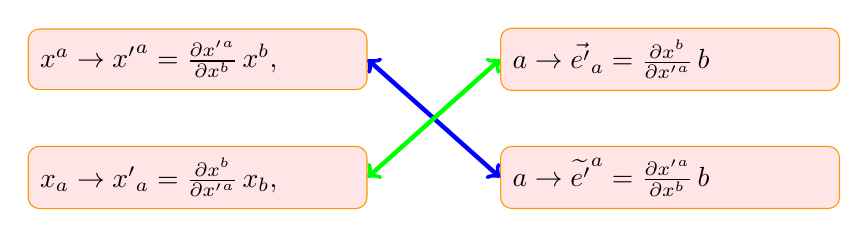
\begin{tikzpicture}
      % Draw the node
      \node[right,text width=4cm,rounded corners,fill=red!10,draw=red!40!yellow,inner sep=1ex] (v)  {$x^a\to {x'} ^a =  \frac{\partial {x'}^a}{\partial x^b} \,x^b,$}; 
      \node[right,text width=4cm,rounded corners,fill=red!10,draw=red!40!yellow,inner sep=1ex,xshift=6cm] (vb) {$\vb{a}\to{\vec{e'}}_a = \frac{\partial {x}^b}{\partial {x'}^a} \,\vb{b}$};
      \node[right,text width=4cm,rounded corners,fill=red!10,draw=red!40!yellow,inner sep=1ex,yshift=-1.5cm] (f) {$x_a\to {x'} _a = \frac{\partial {x}^b}{\partial {x'}^a} \,x_b,$};
      \node[right,text width=4cm,rounded corners,fill=red!10,draw=red!40!yellow,inner sep=1ex,xshift=6cm,yshift=-1.5cm] (fb) {$\fb{a}\to{\widetilde{e'}}^a = \frac{\partial {x'}^a}{\partial {x}^b} \,\fb{b}$}; 
      
      % Draw the connections
      \draw[ultra thick,<->,color=blue] (v.0) -- (fb.180);
      \draw[ultra thick,<->,color=green] (f.0) -- (vb.180);
    \end{tikzpicture}
  \end{center}
  \begin{itemize}
  \item {\color{green!70!black} {\bf covariant} components transform as the vector basis}.
  \item {\color{blue!70!black} {\bf contra-variant} components transform as the dual vector basis}.
  \item They are the inverse of the other.
  \end{itemize}

  \alert{How do the metric transform?}
\end{frame}


\begin{frame}
  \frametitle{Transformation of the Metric}
  The \alert{line-element is a scalar}, i.e., is an invariant under coordinate transformations, therefore,
  \begin{align*}
     {g'}_{cd}\,{x'}^c{x'}^d=& g_{ab} \,x^a x^b\\
    {g'}_{cd}\,\Lambda^c{}_a{x}^a \Lambda^d{}_b{x}^b =& \underbrace{{g'}_{cd}\Lambda^c{}_a\Lambda^d{}_b}_{g_{ab}}\,{x}^a {x}^b
  \end{align*}
Then,
\begin{align*}
  {g'}_{cd} = g_{ab}(\Lambda^{-1})^a{}_c(\Lambda^{-1})^b{}_d.
\end{align*}
\begin{alertblock}{What is this?}
  The metric does not transform as a scalar nor a vector!!!
\end{alertblock}
\end{frame}


\begin{frame}
  \frametitle{Tensors}
  \begin{definition}
    A \alert{\bf Tensor} is a multilinear geometrical  object which transform as,
    \begin{align*}
      T^{a_1\cdots a_p}{}_{b_1\cdots b_q} =  \Lambda^{a_1}_{m_1} \cdots  \Lambda^{a_p}_{m_p}(\Lambda^{-1})^{n_1}_{b_1} \cdots (\Lambda^{-1})^{n_q}_{b_q} {T'}^{m_1\cdots m_p}{}_{n_1\cdots n_q},
    \end{align*}
    i.e., a `vector' transformation per index.
  \end{definition}
  \begin{itemize}
  \item Tensors are classified by their indices, $\binom{p}{q}$-tensors.
  \item Scalars are $\binom{0}{0}$-tensors.
  \item Vectors are $\binom{1}{0}$-tensors, while covectors are $\binom{0}{1}$-tensors.
  \item Metrics are $\binom{0}{2}$-tensors.
  \end{itemize}
\end{frame}


\begin{frame}
  \frametitle{BE AWARE OF ...}
  \begin{alertblock}{WARNING}
    Not every object with indices is a  tensor
  \end{alertblock}
  \begin{example}
    The derivative of a vector is not a tensor,
    \begin{align*}
      \partial_a V^b \;\to \;{\partial'}_a {V'}^b = (\Lambda^{-1})_a^c\, \Lambda^b_d\partial_c\, V^d + \alert{(\Lambda^{-1})_a^c\,\partial_c(\Lambda^b_d) \,V^d }.
    \end{align*}

    In general, it is true for any kind of tensors.
  \end{example}
\end{frame}


\begin{frame}
  \frametitle{Very Special Tensors}
  \begin{itemize}
  \item Kr\"onecker delta: \alert{(Symmetric)}
    \begin{align*}
      \delta_{ab} = 
      \begin{cases}
        1 & a=b\\
        0 & \text{otherwise}
      \end{cases}
    \end{align*}
  \item Levi-Civita epsilon: \alert{(Skew-symmetric)}
    \begin{align*}
      \epsilon_{a_1\cdots a_n} = 
      \begin{cases}
        1 & ({a_1\cdots a_n}) \text{ in an even permutation}\\
        -1 & (a_1\cdots a_n) \text{ in an odd permutation}\\
        0 & \text{otherwise}
      \end{cases}
    \end{align*}
  \end{itemize}
\end{frame}


\begin{frame}
  \frametitle{Vector Algebra in $\R^3$}
  \begin{itemize}
  \item Addition of vectors,
    \begin{align*}
      \vec{V} + \vec{W} = V^i\vb{i}+ W^j\vb{j} = \(V^i +W^i\)\vb{i}
    \end{align*}
  \item Product of a vector 
    with a scalar,% $\lambda\in\K$
    \begin{align*}
      \lambda \vec{V} = \lambda V^i\vb{i} = \(\lambda V^i\)\vb{i}.
    \end{align*}
  \item Scalar product of vectors,
    \begin{align*}
      \vec{V}\cdot\vec{W} = V_i W^i = g_{ij}\; V^i W^j
    \end{align*}
  \item Vector product of vectors,
    \begin{align*}
      \vec{V}\w\vec{W} = \epsilon_{ijk}\;\alert{\fb{i}}\,V^j\, W^k
    \end{align*}
  \end{itemize}
\end{frame}


\begin{frame}
  \frametitle{Vector Calculus in $\R^3$}
  \begin{columns}
    \column{.47\textwidth}
    \begin{itemize}
    \item Nabla: $\widetilde{\partial} = \fb{i}\partial_i$.
      \begin{alertblock}{NOTE:} 
        Nabla is a co-vector, not a vector!
      \end{alertblock}
    \item Gradient:
      \begin{align*}
        \widetilde{\partial}\phi = \fb{i}\partial_i \phi
      \end{align*}
    \item Divergence:
      \begin{align*}
        \widetilde{\partial}\vec{V} =& \fb{i}\partial_i \(V^j\,\vb{j}\)\\
        =& \fb{i}\(\vb{j}\)\,\partial_i V^j\\
        =& \partial_i V^i.
      \end{align*}
    \end{itemize}
    \column{.47\textwidth}
    \begin{itemize}
    \item Curl: 
      \begin{enumerate}[i]
      \item It's only defined in 3-dimensions.
      \item In general act on co-vectors.
      \item The result is \alert{not} a vector!!!
      \end{enumerate}
      \begin{align*}
        \widetilde{\partial}\w\widetilde{V} = \(\partial_i V_j - \partial_j V_i\)\fb{i}\otimes\fb{j}
      \end{align*}
    \end{itemize}
  \end{columns}
\end{frame}


\begin{frame}
  \frametitle{Manifolds}
  \begin{definition}
    A \alert{\bf Manifold}, $\Mi$, is a space locally homeomorphic to $\R^n$, for some $n$. The dimension of $\Mi$ is $n$.
  \end{definition}
  \begin{columns}
    \column{.5\textwidth}
    \begin{center}
      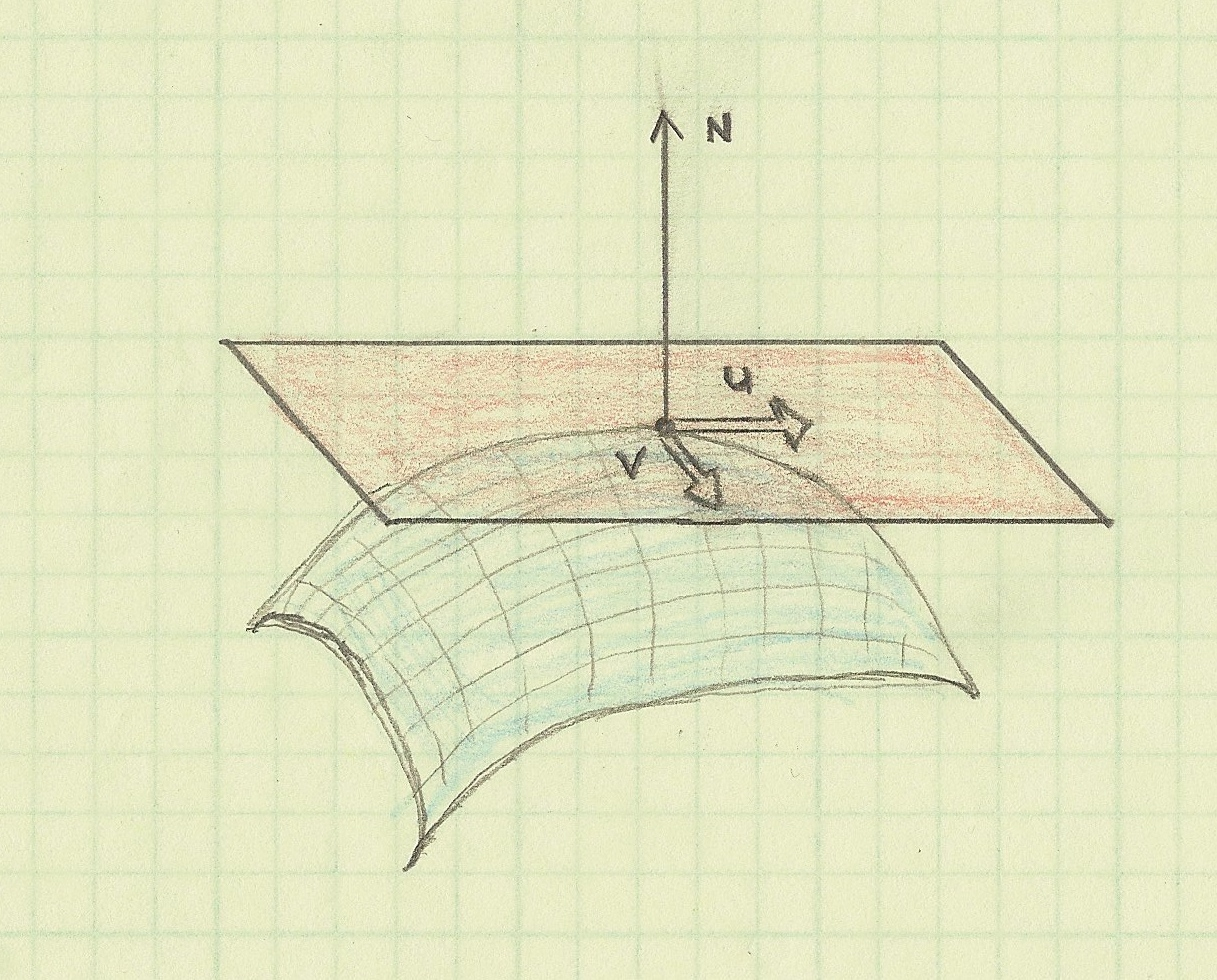
\includegraphics[scale=.11]{Pict/Tang-vect2.jpg}
    \end{center}
    It \alert{is} a 2-dimensional manifold.
    \column{.5\textwidth}
    \begin{center}
      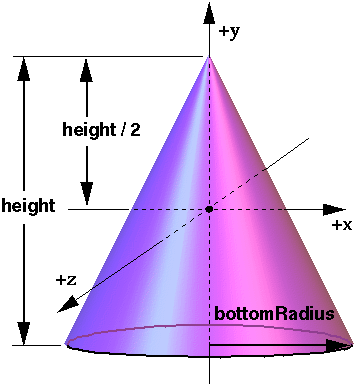
\includegraphics[scale=.3]{Pict/cone.png}
    \end{center}
    It \alert{is NOT} a 2-dimensional manifold.
  \end{columns}
\end{frame}

\begin{frame}
  \frametitle{How are vectors defined on a manifold?}
  \begin{columns}
    \column{.5\textwidth}
    On a 2-sphere:
    \begin{itemize}
    \item The vector (arrow) does not belong to the sphere (?!)
    \item The only point who touch the manifold is the tail
    \item The set of vector passing through a point $p$, form a tangent space.
    \end{itemize}
    \column{.5\textwidth}
    \begin{center}
      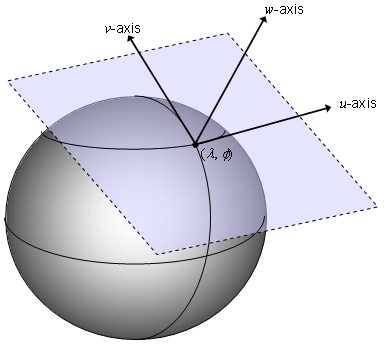
\includegraphics[scale=.4]{Pict/TanSphere.jpg}
    \end{center}
  \end{columns}

  \begin{alertblock}{Vectors on Manifolds}
    Since the tangent space is flat, vectors on a manifold are defined on the tangent space.
  \end{alertblock}
\end{frame}


\begin{frame}
  \frametitle{Tangent... What???}
  Since the tangent space, $T_p\Mi$, is defined at a point $p$, in order to define vector on the whole of the manifold, one needs the collection of all tangent spaces, $$T\Mi = \amalg_p\, T_p\Mi.$$
  \begin{definition}
    The collection of all tangent spaces is called \alert{\bf Tangent Bundle}, $T\Mi$.
  \end{definition}

  Similarly, for the covectors.
  \begin{definition}
    A cotangent space at $p$, $T^*_p\Mi$, is the tangent space spanned by the tangent covectors at $p$. The collection of all cotangent spaces, $T^*\Mi$ is called \alert{\bf Cotangent Bundle}.
  \end{definition}
\end{frame}

\begin{frame}
  \frametitle{Mind-map of Bundles}
  \begin{center}
    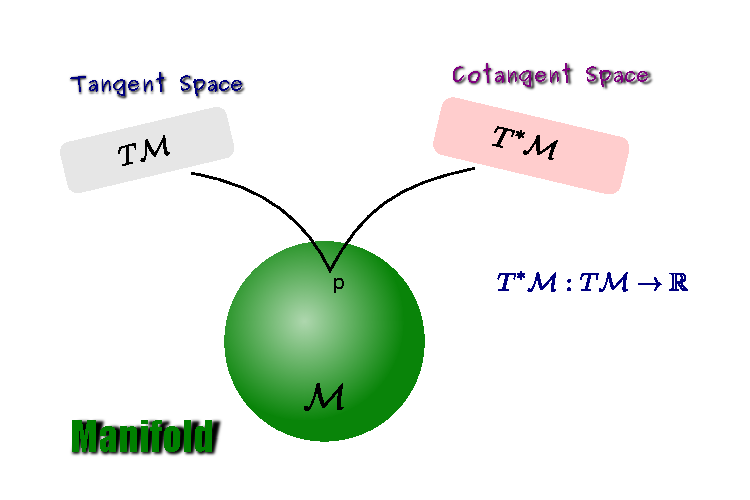
\includegraphics[scale=.9]{Pict/Tan-Cotan.pdf}
  \end{center}
\end{frame}

\begin{frame}
  \frametitle{Comparing vectors}
  If  $\vec{V}\in T_p\Mi$ and $\vec{W}\in T_q\Mi$, How does one know if $\vec{V}\neq \vec{W}$?

  \begin{columns}
    \column{.6\textwidth}
    \begin{center}
      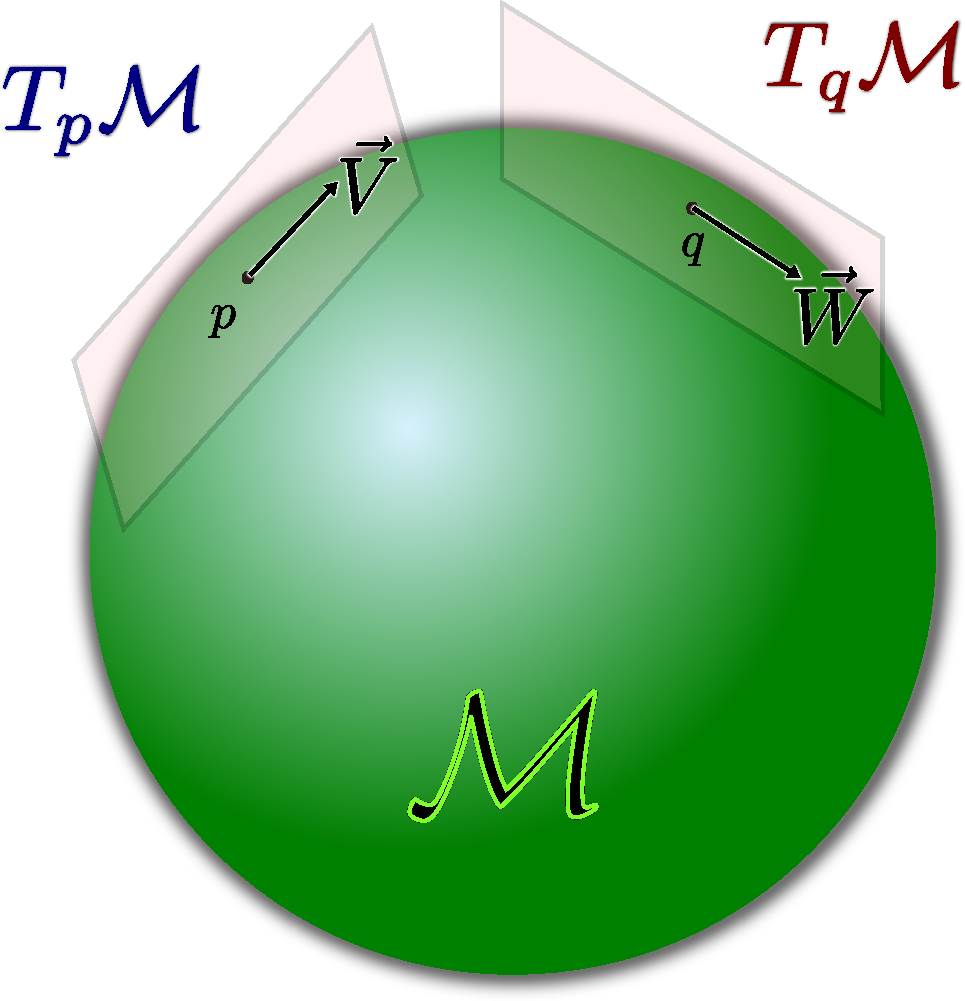
\includegraphics[scale=.35]{Pict/Compare.pdf}
    \end{center}
    \column{.4\textwidth}
    In order to compare one needs to drag one vector to the tangent space of the other.

    This procedure is known as \alert{Parallel Transport}
  \end{columns}
\end{frame}

\begin{frame}
  \begin{columns}
    \column{.45\textwidth}
    \frametitle{Parallel Transport and Connections}
    In order to parallel transport one needs:
    \begin{itemize}
    \item \alert{A path}: joining the point $p$and $q$.
    \item \alert{A connection}: a geometrical object which tells who a tangent space  is related with the one in its neighbourhood.
    \end{itemize}
    \column{.45\textwidth}
    \begin{alertblock}{Levi-Civita Connection}
      A very useful connection is the Levi-Civita connection, $\Gamma^a_{bc}$, which defines how the vector basis changes if one moves along a certain direction.$$\nabla_b \vb{c} = \Gamma^a_{b c}\,\vb{a}.$$
    \end{alertblock}
  \end{columns}

  \begin{block}{Covariant Derivatives}
    A connection allows to define a covariant derivative, which assures that the obtained object transforms as a tensor.
  \end{block}
\end{frame}

\begin{frame}
  \frametitle{Curvature}
  In general the commutation of parallel transportation along non co-lineal directions does not vanishes. The failure of this commutation is known as the \alert{curvature} of the ``manifold''.

$$\comm{\nabla_a}{\nabla_b}V^c= \Ri_{a b}{}^c{}_d V^d,$$
and $\Ri_{a b}{}^c{}_d$ is the Riemman tensor.

The Ricci tensor is defined by,$$\Ri_{a b}= \Ri_{c a}{}^c{}_b.$$

And the Ricci scalar,
\begin{align*}
  \Ri = \Ri_{ ab}\, g^{ab}.
\end{align*}
\end{frame}

\begin{frame}
  \frametitle{General Tensors}
  \begin{definition}
    A type $\binom{p}{q}$ tensor is a geometrical object which belongs to a bundle,
    \begin{align*}
      T^{a_1\cdots a_p}{}_{b_1\cdots b_q}\in \(\otimes^p T\Mi \)\otimes\( \otimes^q T^*\Mi\).
    \end{align*}
  \end{definition}

  \begin{itemize}
  \item \underline{\sc Contraction:}\hspace{1cm} $\delta:\binom{p}{q}\to\binom{p-1}{q-1}.$
  \item \underline{\sc Derivation:}\hspace{1.3cm} $\nabla:\binom{p}{q}\to\binom{p}{q+1}$.
  \item \underline{\sc Addition:}\hspace{1.7cm} $+:\binom{p}{q}\times\binom{p}{q}\to\binom{p}{q}$.
  \item \underline{\sc Tensor Prod.:}\hspace{.8cm} $\otimes:\binom{p_1}{q_1}\times\binom{p_2}{q_2}\to\binom{p_1+p_2}{q_1+q_2}$.
  \item \underline{\sc \alert{Contraction}:}\hspace{1cm} $\delta:\binom{p_1}{q_1}\times\binom{p_2}{q_2}\to\binom{p_1+p_2-1}{q_1+q_2-1}$.
  \item And much more...!!!
  \end{itemize}
\end{frame}

{\usebackgroundtemplate{
    
\includegraphics[width=\paperwidth,
      height=\paperheight]{Pict/darthvader30.pdf}
  }
\begin{frame}
  \frametitle{Conclusions}
  \begin{itemize}
  \item Differential Geometry is a vast subject.
  \item Not all of the differential geometry is as simple as in $\R^n$.
  \item There are tangent spaces... Lots of them!!!
  \item The introduction of a connection is necessary.
  \item When taking about geometrical objects on manifolds, people mean on \alert{Bundles}.
  \item We shall come back to all this with further detail.
  \end{itemize}
\end{frame}
}
